% Figure 10 -- a) U(1)xU(1) with n-2 bifundamentals; b) the regular puncture legs;
%              c) U(2) split into two U(1); d) after gluing
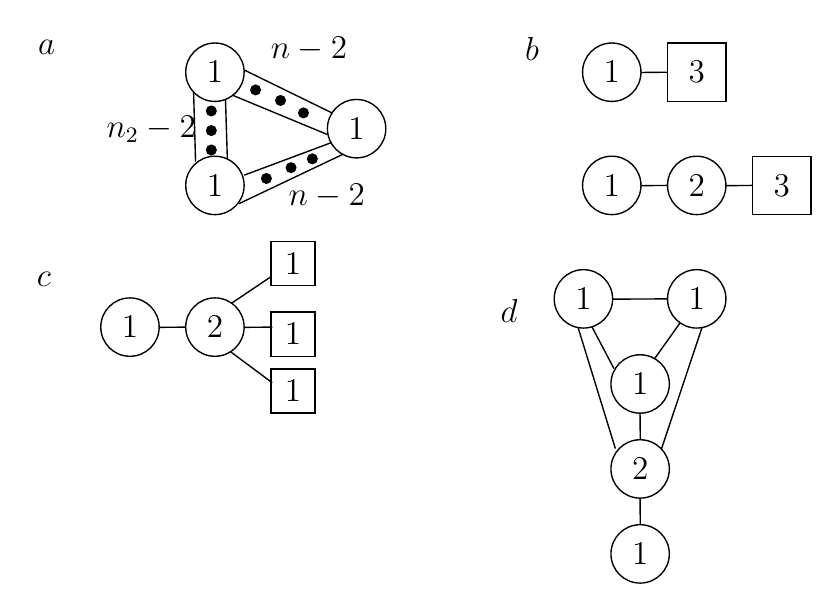
\begin{tikzpicture}[x=1pt,y=1pt,>=stealth,line width=0.5pt,
    nd/.style={circle,draw,fill=white,inner sep=0pt,minimum size=21.1pt,
               font=\fontsize{11.5}{14}\selectfont},
    sq/.style={rectangle,draw,fill=white,inner sep=0pt,minimum width=21.2pt,
               minimum height=21.1pt,font=\fontsize{11.5}{14}\selectfont},
    rr/.style={font=\fontsize{11.5}{14}\selectfont}]
  % =================== a) ===================
  % ribbon between the two left nodes (vertical)
  \draw (65.2,188.5) -- (65.9,163.5);
  \draw (76.7,186.6) -- (77.4,164.1);
  % ribbon to the right node, upper
  \draw (79.0,187.6) -- (113.5,173.3);
  \draw (83.5,196.6) -- (115.4,181.0);
  % ribbon to the right node, lower
  \draw (81.6,148.3) -- (119.9,166.5);
  \draw (83.5,158.6) -- (114.8,170.3);
  \foreach \x/\y in {91.5/157.4, 100.4/161.3, 108.1/164.5,
                     71.6/167.7, 71.6/174.7, 71.6/181.8,
                     104.9/181.1, 96.6/185.6, 87.6/189.4}
    {\fill (\x,\y) circle[radius=2.0pt];}
  \node[nd] at (72.9,195.8) {1};
  \node[nd] at (72.9,154.9) {1};
  \node[nd] at (124.1,175.4) {1};
  \node[rr] at (106.9,204.2) {$n-2$};
  \node[rr] at (113.3,151.1) {$n-2$};
  \node[rr] at (49.9,175.2) {$n_2-2$};
  \node[rr] at (12.1,204.8) {$a$};
  \node[rr] at (187.5,204.2) {$b$};
  % =================== b) ===================
  \draw (226.2,195.7) -- (237.1,195.8);
  \node[nd] at (216.3,195.8) {1};
  \node[sq] at (247.0,195.85) {3};
  \draw (226.2,154.8) -- (237.1,154.9);
  \draw (256.9,154.8) -- (267.8,154.9);
  \node[nd] at (216.3,154.9) {1};
  \node[nd] at (247.0,154.9) {2};
  \node[sq] at (277.75,154.85) {3};
  % =================== c) ===================
  \draw (52.1,103.6) -- (63.0,103.7);
  \draw (82.8,103.6) -- (93.7,103.7);
  \draw (78.4,94.9) -- (93.6,83.6);
  \draw (79.0,112.4) -- (93.0,121.8);
  \draw (93.1,118.7) rectangle (109.1,134.7);
  \draw (93.1,93.1) rectangle (109.1,109.1);
  \draw (93.1,72.6) rectangle (109.1,88.6);
  \node[nd] at (42.2,103.7) {1};
  \node[nd] at (72.9,103.7) {2};
  \node[rr] at (101.1,126.7) {1};
  \node[rr] at (101.1,101.1) {1};
  \node[rr] at (101.1,80.6) {1};
  \node[rr] at (11.1,121.0) {$c$};
  % =================== d) ===================
  \draw (216.0,113.8) -- (237.1,113.9);
  \draw (208.4,105.2) -- (217.1,88.7);
  \draw (231.5,91.9) -- (241.4,105.8);
  \draw (203.4,105.9) -- (217.6,59.8);
  \draw (234.1,59.2) -- (249.7,105.9);
  \draw (226.5,73.9) -- (226.6,63.0);
  \draw (226.5,43.8) -- (226.6,32.3);
  \node[nd] at (206.05,113.9) {1};
  \node[nd] at (247.0,113.9) {1};
  \node[nd] at (226.55,83.15) {1};
  \node[nd] at (226.55,52.45) {2};
  \node[nd] at (226.55,21.75) {1};
  \node[rr] at (179.2,109.5) {$d$};
\end{tikzpicture}
